%%%%%%%%%%%%%%%%%%%%%%%%%%%%%%%%%%%%%%%%%%%%%%%%%%%%%%%%%%%%%%%%%%%%%%%%%%%%%%%%
% simulation.tex: Chapter on MC production:
%%%%%%%%%%%%%%%%%%%%%%%%%%%%%%%%%%%%%%%%%%%%%%%%%%%%%%%%%%%%%%%%%%%%%%%%%%%%%%%%
\chapter{Simulation}
\label{simulation_chapter}
%%%%%%%%%%%%%%%%%%%%%%%%%%%%%%%%%%%%%%%%%%%%%%%%%%%%%%%%%%%%%%%%%%%%%%%%%%%%%%%%

%%%%%%%%%%%%%%%%%%%%%%%%%%%%%%%%%%%%%%%%%%%%%%%%%%%%%%%%%%%%%%%%%%%%%%%%%%%%%%%%
In order to predict spectra at the near and the far detectors to compare predictions with
actual data one need to simulate neutrino interactions in the detectors relying on
known physics models and theories of how particles are produced, how they travel and interact
with detector material. The simulation process in the NOvA starts with protons hiting
NuMI target and finishes with APD readouts and analog to digital converters. Side simulation
packages or custom NOvA software are used in every step, output information on every step is
used as input data for the following step
\begin{itemize}
\item Beam simulations. FLUGG simulation package which is the combination of FLUKA \cite{FLUKA} 
and GEANT4 \cite{GEANT4} packages. Geometries of the target hall and detectors are encoded with 
the help of GEANT4, while proton interactions and downstream particle decays are simulated with FLUKA.
\item Neutrino interactions. Neutrino flux degenrated in the previous step is an input for
the GENIE \cite{GENIE} package, which performs simulation of neutrino interactions with nucleus inside the
detectors. GENIE produces a list of particles leaving the nucleus.
\item Propagation of particles through detectors. List of the particles and detailed detectors geometry are
used by GEANT4 to simulate particles propagation through the detectors. Amount of energy deposited
by the particles in every cell is the input for the last step.
\item Electronic signal. Deposited energy in the cell is converted to a light by the scintillator
which travels through the fiber to an APD and analog to digital converter. This step is
simulated by NOvA custom software \cite{NovaSim}.
\end{itemize}
All these 4 parts will be briefly discussed in the current chapter.

\section{Beam Simulation}
Beam simulation provides NOvA experiment with neutrino flux prediction at both detectors. 
This simulation is done by FLUKA and GEANT4 through the FLUGG interface. Detailed geometry of
the target hall, target itself, collimator, two focusing horns and decay pipe is described by
GEANT4 format files and simuation is done by FLUKA. The FLUKA package simulates 120 GeV protons
which hit the target and give rise to hadronic showes, secondary particles focused by the horns 
and enter decay pipe where they further decay and some of them produce neutrinos. All the proton 
interaction information whose dauther particles produce neutrino is saved providing a way to 
study beam uncertanties related to particle production models. 

The simulation outputs files which describe neutrino flux in terms of neutrino parent particles, 
flavour, energy and direction of motion.

\section{Simulation of Neutrino Interactions}
In order to simulate neutrino interactions in the near and far detector the GENIE simulation 
package is used. The package is developed by the experimental physics community and serves as a 
primary neutrino Monte Carlo generator for neutrino experiments due to its ability to simulate neutrino
interactions on almost any target and in wide energy region which spans from MeV to PeV. As mentioned 
above GENIE gets a result of neutrino flux simulation from a previous step and convolute it with
neutrino interaction cross sections.

The interesting feature of the neutrino energy spectrum in NOvA experiment is that it overlaps 
with energy regions of several neutrino interaction models. All these models are implemented in GENIE
simulation package. Quasi-Elastic scattering (QE), deep-inelastic scattering (DIS), baryon resonance 
production (RES) as well as meson exchange current (MEC) which dominates in 2 particle - 2 hole (2p-2h) 
effect. The physics behind the models is complicated, however on the qualitative level QE interaction 
means scattering off a single nucleon, MEC interaction means scattering off a pair of nucleons, RES process
results in excitation of the whole nucleus and DIS interaction of neutrino with a nucleus can lead to a 
complete disintegration of the nucleus\footnote{This happens when energy transferred to a nucleus is 
sufficiently large}.

\begin{figure}[t!]
\begin{subfigure}[t]{.5\textwidth}
  \centering
  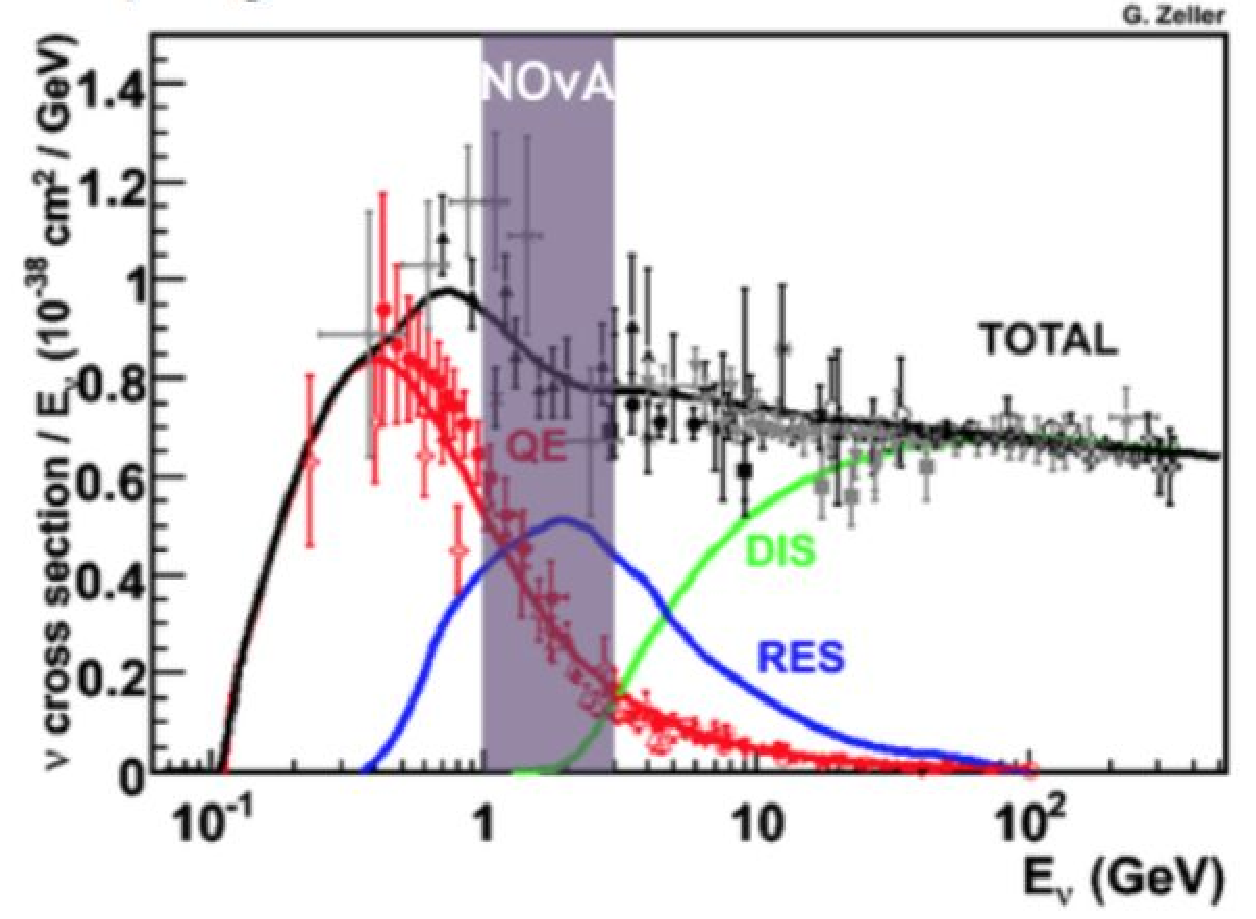
\includegraphics[width=0.85\linewidth]{figures/nu_channels.pdf}
  \caption{Neutrino cross section energy dependence for QE, RES and DIS intercations overlapped with 
	NOvA energy region used for the oscillation analysis.}
  \label{fig:NovaEReg}
\end{subfigure}%
~
\begin{subfigure}[t]{.5\textwidth}
  \centering
  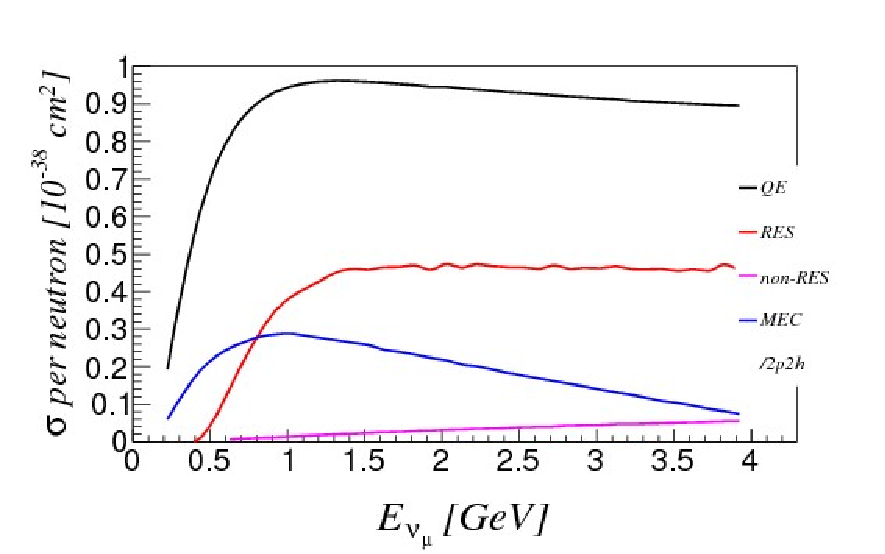
\includegraphics[width=1.1\linewidth]{figures/mec_xsec.pdf}
  \caption{Neutrino cross section energy dependence used in GENIE neutrino generator.}
  \label{fig:mecXsec}
\end{subfigure}
\caption{Neutrino cross sections.}
\label{fig:simPlots}
\end{figure}

On the left hand side of \ref{fig:NovaEReg} one can see a typical energy regions of QE, RES and DIS neutrino 
interactions overlaped with NOvA energy domain. These three types of neutrino scattering are implemented 
in GENIE based on the Llewellyn-Smith model \cite{QE}, Rein-Sehgal model \cite{RES} and effective leading 
order model with Bodek and Yang modifications \cite{DIS} for QE, RES and DIS respectively. MEC process, 
which is included in GENIE as semi-empirical model, is described in \cite{MEC}.

\section{Particles propagation}
After GENIE is done with its part of simulation, or in other words, the list of particles which leave 
the nucleus with their energies, momenta and initial positions is ready, now one needs to propagate them
through the detector material and simulate the energy deposition, interaction and decay. NOvA experiment
uses GEANT4 \cite{GEANT4} simulation package for this step. Besides the list of particles, GEANT4 takes
another input namely geometry of the detector and its surrounding. Detailed information about blocks 
positions, cell structure and materials they made of, scintillator composition, conrete and steel support
structure around the detectors is encoded in special geometry files.

The way GEANT4 propagates particles is done in the following manner. For each particle at each step of the 
trajectory it is decided with appropriate probability what particle should do next - move forward and deposit 
some energy, interact and scatter of particles which constitute detector components or decay. As particle
propagates further it loosing its kinetic energy and as soon as particle's kinetic energy is less than 100 eV
propagation stops. GEANT4 saves these trajectory steps as a list of particle positions, energy and momenta 
for the next step of simulation chain. 

Before the final detector response could be simulated it is necessary to determine how much light was produced
in the scintillator and what fraction of it was collected by the wave-shifting fiber and transported to the 
readout electronics. As a matter of fact, amount of light produced by the scintillator is not linearly 
proportional to amount of deposited energy due to a finite number of scintillaotr centres along the particle
trajectory in the cell. The effect is know as Birks supression \cite{birks}. If $\frac{dL}{dx}$ is light 
output per unit length and $\frac{dE}{dx}$ is amount of deposited energy then Birks law reads
\be
\frac{dL}{dx} = L_0 \frac{\frac{dE}{dx}}{1 + k_B\frac{dE}{dx}}, 
\ee
where $L_0$ and $k_B$ are constants which depend on scintillator. However, more carefull aproach to the problem
of particle propagation through scintillator was carried out by Chou \cite{chou} and additional correction was
introduced to the Birks law. NOvA experiment utilizes this correction - 
\be
\frac{dL}{dx} = L_0 \frac{\frac{dE}{dx}}{1 + k_B\frac{dE}{dx} + k_C\Big(\frac{dE}{dx}\Big)^2}.
\ee
Parameters $k_B$ and $k_C$ are tuned using muon and protons tracks in the Near Detector.

\section{Light propagation and signal to store}
The last step in simulation is done with custom NOvA software and could be split into two parts - light 
propagation to the readout electronic and signal forming by that electronic. While on practice cells could 
be different from each other (horizontal cells are not exactly horizontal because of their length - cells could be
slightly bent, escpecially in the far detector. Not exact horizontality also leads to small bubbles of air are
being trapped inside the cells) it is assumed in simulation that all the cells are exactly the same.

\subsection{Light propagation}
Assumption that all cells are equivalent and usage of ray-tracing model allow to find a template to determine how 
many photons were trapped by the wave-shifting fiber. Following characteristics of detector components were 
measured in bench experiments 
\begin{itemize}
\item characteristic scintillator emission time - 9 ns
\item scintillator index of refraction - 1.46
\item reflectivity of the cell walls - 87.7\%
\item capture length of photon capture probability\footnote{Probability to capture a photon $P \sim e^{x/L}$, where
$x$ is distance between the point where the photon was produced and the fiber, $L$ is capture length.} - 30.66 cm
\end{itemize}
The resulting template is shown on \ref{fig:Coll_rate}. Knowing how many and where photons were emitted and using
the template number of trapped photons could be determined. To simulate what fraction of photons reaches the APD
half of photons are sent in opposite directions around the fiber. There are some fraction on photons which is 
absorbed or get out of fiber and in order to account for that simulation uses attenuation curve which was 
measured in bench tests. Before the last phase of simulation starts number of photoelctron created in the APD
is determined by taking into account APD's quantum efficiency and additional Poisson smearing.
\begin{figure}
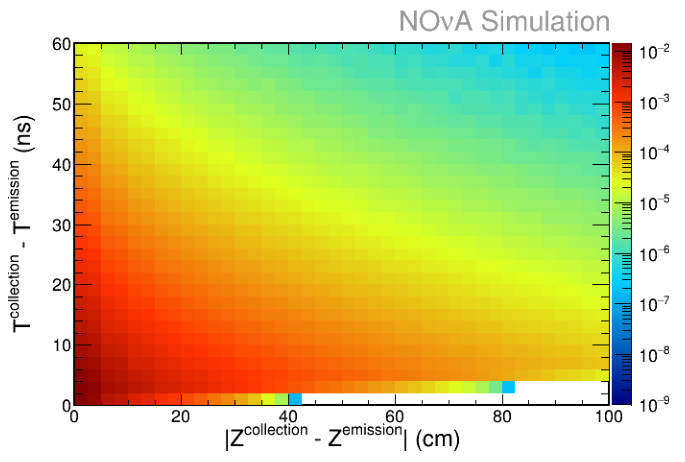
\includegraphics[width=1.0\textwidth]{figures/Coll_rate.png}
\centering
\caption{The collection rate of scintillator photons by a wavelength shifting fiber loop relative to the position 
	and time where and when the energy was deposited.} \label{fig:Coll_rate}
\end{figure}
\begin{figure}[t!]
\begin{subfigure}[t]{0.9\textwidth}
  \centering
  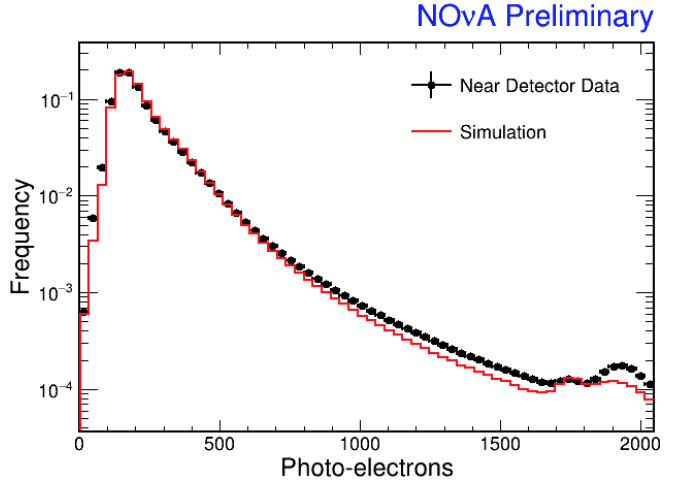
\includegraphics[width=0.9\linewidth]{figures/AttenuationND.png}
  \caption{Near Detector}
  \label{fig:attND}
\end{subfigure}
\vspace{0.5cm}
\newline
\begin{subfigure}[t]{0.9\textwidth}
  \centering
  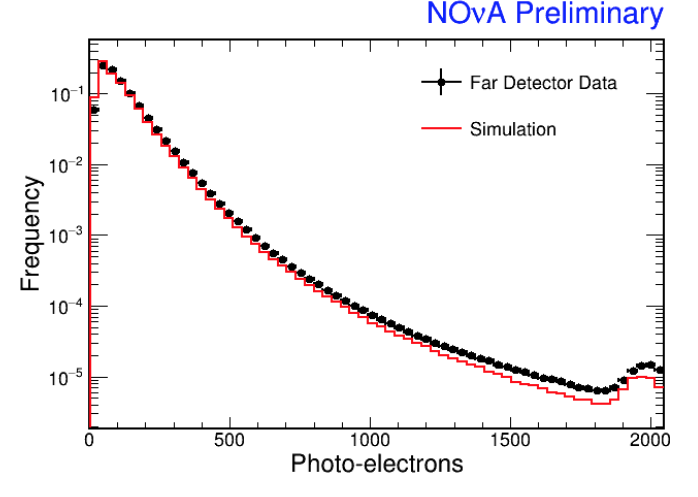
\includegraphics[width=0.9\linewidth]{figures/AttenuationFD.png}
  \caption{Far Detector}
  \label{fig:attFD}
\end{subfigure}
\caption{Attenuation curves for the near and the far detectors. Data points are detectors response to cosmic ray
	muons while simulation curves are results of bench experiments.}
\label{fig:att}
\end{figure}

\subsection{Electronics}
\begin{wrapfigure}{r}{0.5\textwidth}
\vspace{-20pt}
  \begin{center}
    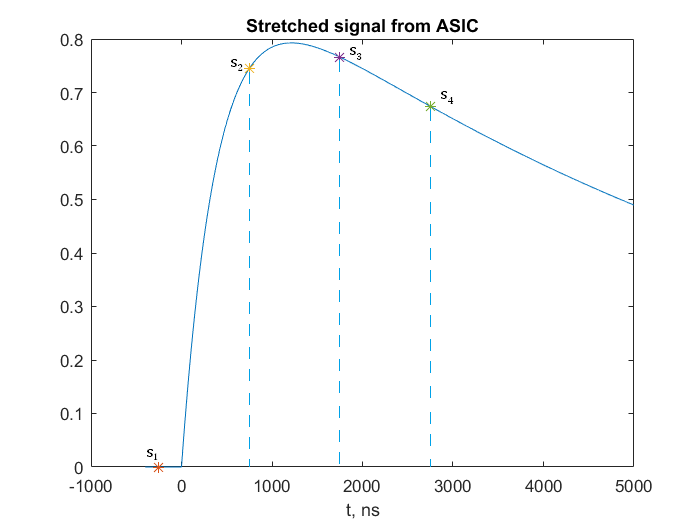
\includegraphics[width=0.48\textwidth]{figures/digit_scheme.png}
  \end{center}
\vspace{1mm}
\caption{Schematics of digitization}
\end{wrapfigure}
Photo-electron signal in the APD created in the previous step have to be digitazed to finalize the simulation
of the cell hit. As APD impulse is too short, first it is stretched in the Application Specific Integrated 
Circuit (ASIC) by CR-RC circuit. The response of the ASIC to a charged impulse has the following form
\be
f(t) \sim e^{-\frac{t-t_0}{F}} - e^{-\frac{t-t_0}{R}},
\ee
where $t_0$ is the time when pulse was created by APD, F and R are the fall time and rise time of the CR-RC 
circuit. And as was mention in chapter \ref{experiment_chapter} the signal value is split into 4096 possible
values and only 4 last ADCs - value of the digitization sample - is stored when the difference $ADC_i - ADC_{i-3}$
is greater then a treshold. 
At this point simulation files have the same structure\footnote{Of course plus additional information about type 
of neutrino information, resulting particles' momenta and energies etc.} as files with detectors gathered data.
The next step in NOvA analysis is to reconstruct high level information about recorded or simulated events
with the help of reconstruction algorithms which are the same for the real data and simulation.
